\documentclass[12pt]{article}

% Useful packages
\usepackage[utf8]{inputenc}
\usepackage{fullpage}
% \usepackage{times}
\usepackage{setspace}
\usepackage{biblatex}
\usepackage{amsmath}
\usepackage{graphicx}
\usepackage{pdfpages}
\usepackage{float}
\usepackage[colorlinks=true, allcolors=blue]{hyperref}

% bibliography
\addbibresource{references.bib}

\title{Finding the Shortest Paths in the University of Minnesota Minneapolis Campus Map}
\author{Junyuan Wang, Yicheng Zhai}

\begin{document}
\maketitle

\begin{abstract}
To aid walkers in navigating their ways within the campus of the University of Minnesota Twin Cities, we developed a navigation program that offers a selection of algorithms, namely A* with Manhattan, A* with Haversine, Breadth-First Search, Bidirectional Search, Dijkstra Algorithm, and Bellman-Ford Algorithm. Our results show that the Bellman-Ford Algorithm delivers the optimal route, but it exhibits an exceedingly high run-time and memory usage. In contrast, the Dijkstra Algorithm produces a marginally inferior route but utilizes fewer resources. The Breadth-First Search and Bidirectional Search algorithms require less time and space in comparison to the previous two algorithms, however, their routes are less satisfactory. The two variations of A* were determined to be unsuitable for this particular map, as the overall performance is inferior to that of the aforementioned algorithms. 
\end{abstract}


\section{Introduction}

Within the expansive campus of the University of Minnesota (UMN), strategic route planning assumes utmost significance for students who must navigate between academic buildings to attend classes. In practicality, students frequently encounter the need to traverse considerable distances across the campus in a time-constrained manner, typically within a tight time frame of 15 minutes, to reach the designated teaching building where their next course is scheduled. In contrast to conventional navigation methods, We aim to develop a more optimized program with multiple algorithms to facilitate efficient route planning for students, subsequently evaluating the comparative performance and efficiency of various search algorithms in this program.

We extract data from OpenStreetMap (OSM) to meticulously construct a 2D campus map of the University of Minnesota. This map was seamlessly integrated into a web page providing users with an interactive and visually appealing interface (Figure \ref{fig: map ui}). Within this interface, users can select a start, a destination, and the algorithm they want to use to calculate the optimal path between these two points on the map.

Through the utilization of Python programming language along with its robust NetworkX library, we can leverage various algorithms to determine the optimal path between two points on a given map. In our algorithm selection process, we prioritized the utilization of efficient algorithms that have proven effective in solving similar problems. These include the widely-used A* algorithm, the classic Dijkstra's algorithm, the Breadth-First search algorithm, the Bidirectional search algorithm, and the Bellman-Ford algorithm.

This paper will discuss the implementation of the program and evaluate the performance of the aforementioned algorithms on the University of Minnesota map. The paper is structured as follows. Section 2 covers a literature review of the tools and algorithms used in this project. Section 3 delineates the process of implementing the program and the references for the algorithms. Section 4 documents the design and results of the algorithm performance comparison experiment, which incorporates an in-depth analysis of the results. Section 5 gives the concluding remarks for the project. Finally, Section 6 delineates the specific division of labor involved in the project.


\begin{figure}[ht]
\centering
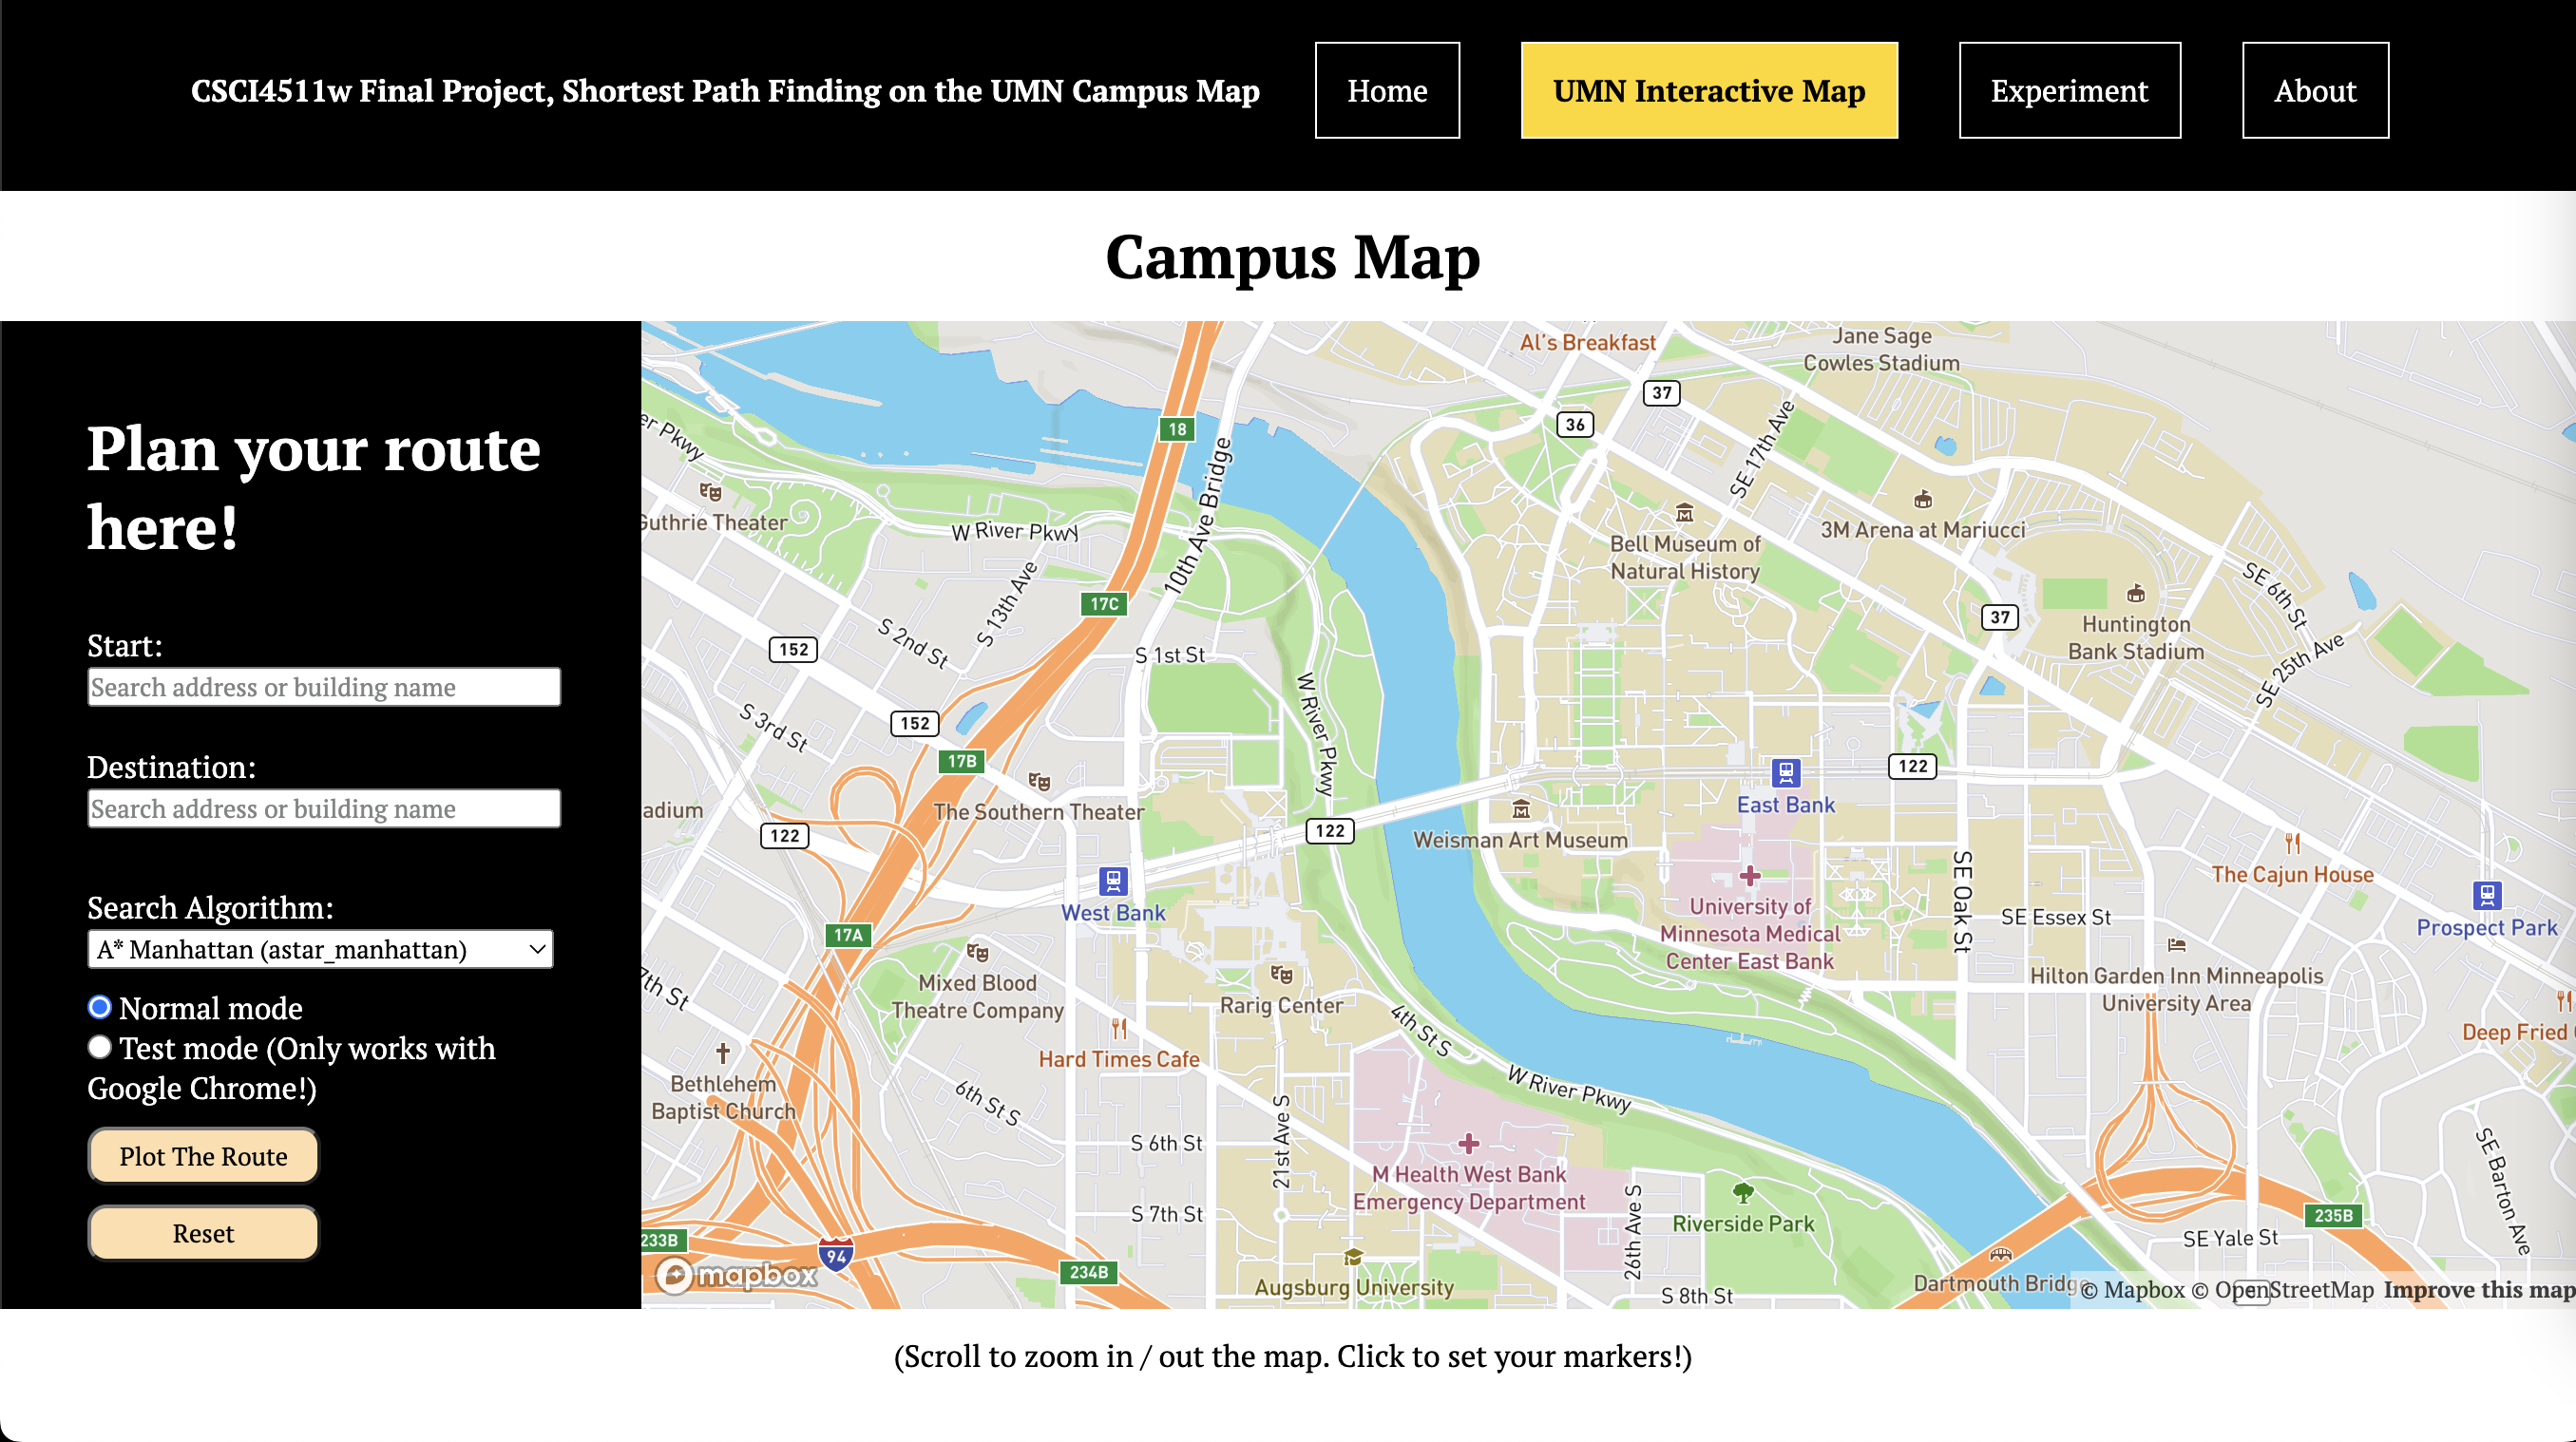
\includegraphics[scale=0.3]{images/map_ui.png}
\caption{The user interface of the UMN Interactive Map}
\label{fig: map ui}
\end{figure}


\section{Background Knowledge}

Since this project aims to help users find the shortest path within the UMN Twin Cities campus by utilizing OpenStreetMap (OSM), NetworkX, and Python, along with algorithms including A* and Dijkstra’s algorithms, the background knowledge is separated into three parts. First, it will introduce these tools and algorithms by providing an overview of their key features and capabilities and explore how these methods have been employed in similar studies when solving real-world path-finding problems. Second, it will examine other studies using similar algorithms to ours. Finally, it will summarize the experimental approaches and conclusions derived from these studies.

\subsection{Tools}

\subsubsection{OSM}

Given that this project relies on map data from OpenStreetMap (OSM), we need to assess the trustworthiness of the data. Grinberger’s study \cite{Grinberger_Minghini_Juhász_Yeboah_Mooney_2022} offers an academic perspective on evaluating the reliability of OSM data, focusing on three perspectives of OSM data: Application of OSM data, OSM data quality, and Dynamics in OSM. The study highlights the impressive scale of the project, with almost 7.5 billion data nodes contributed by 1.8 million users as of March 2022. It is also common to see scholars incorporate OSM data by contributing mapping resources into more advanced models, especially machine learning. The analysis of OSM data quality provides evidence of a fair accuracy of OSM data on tourism. However, since the OSM data is ”crowd-sourced”, i.e., the communities might have different ways of communication and evaluations of science, the article points out that it requires more understanding to utilize OSM data. In light of these findings, we are confident in the reliability of OSM data, though we might spend more time on data processing.

\subsubsection{NetworkX, Python (PyCharm)}

To improve the efficiency of data manipulation and the quality of data visualization, the project will utilize NetworkX as an important tool while implementing our algorithms in Python programming language which is easy to code and document. In Hagberg’s article \cite{Hagberg_Aric_Pieter_Daniel_2008}, it introduces how flexible NetworkX is when representing different types of graphs, edges, and nodes that are fundamental for networks like ours. Beyond this, NetworkX also provides many functions to calculate the statistics of the network like connected nodes, coefficient, etc. By utilizing the ”dictionary of dictionaries” as its basic data structure for graphs, NetworkX facilitates finding the shortest path in a weighted graph and simplifies the algorithms required for this project. Additionally, NetworkX supports the integration of external tools, allowing us to incorporate more tools like Graphviz and Matplotlib into NetworkX to generate more detailed visualizations for the project.

\subsection{Algorithms}

\subsubsection{A*}

As A* and Dijkstra are two common algorithms to discuss and be implemented by scholars, Aziz \cite{Aziz_Anusha_Sheikh_2022} conducted an experiment using a 25x25 grid-based environment to compare the performances of A*, Ant Colony Optimization (ACO), and Dijkstra’s Algorithms. Despite the limitations of the experiment, such as the distancing problem and different characteristics of the three algorithms, A* is shown to win the game.

Zeng \cite{Zeng_Church_2009} performed an empirical study on road network data in California, demonstrating that “on real road networks, A* outperforms the best implementations of the Dijkstra algorithm by a significant margin.” The superior performance of A* was achieved through the use of spatial coordinates to refine the search for the shortest path. The authors note that the potential of the A* algorithm can be further enhanced by improving its heuristic function. By generating more accurate estimated completion costs, the number of visited nodes and algorithm run-time can be reduced. This observation highlights the flexibility of the A* algorithm and motivates us to improve the A* algorithm for achieving better performance in this project.

\subsubsection{Dijkstra}

Analogous to our project, the self-driving automobile proposed in He’s application \cite{He_2022} of Dijkstra’s algorithm in finding the shortest path shares the same objective, but with the added dimension of determining the shortest distance between two regions. The authors have directed their focus towards the utilization of Dijkstra’s algorithm and posited that ”Dijkstra algorithm is faster than other algorithms for it can calculate the shortest length to every point”. The algorithm employs a pyramid tree structure to pinpoint all vertex nodes that fall within the range of interest, as well as a heap to preserve distances and extract nodes with the least distance. These salient features impel us to prioritize testing and deploying Dijkstra’s algorithm in our research project.

Fitro’s experiment \cite{Fitro_2018} which incorporates Geographic Information System (GIS), Google Map API, and Dijkstra’s algorithm to find the shortest path at Taman Subdistrict, Indonesia, mentions that Dijkstra’s algorithm spends a large memory space. In the experiment, the author introduces a node combination technique to reduce memory usage, i.e., ”merging two nodes that have the closest distance”, and the optimal paths are shown in the result.

Wayahdi \cite{Wayahdi_2021_GreedyAA} presents a further comparative analysis of the efficiency of Greedy, A*, and Dijkstra, for determining the shortest path in a given graph. The Greedy algorithm, while speedy, may not necessarily guarantee a solution. On the other hand, the A* algorithms are relatively more efficient, but their performance is contingent upon complex data. In contrast, the Dijkstra algorithm invariably produces the optimal outcome, making it the ideal choice for shortest path determination. However, it may take longer to solve the problem than the other two algorithms. Despite this drawback, the author unequivocally recommends employing the Dijkstra algorithm for solving problems involving complex searches for determining the shortest path.

\subsubsection{Bellman-Ford}

The Bellman-Ford algorithm is also widely utilized for solving the problem of identifying the shortest path between two points. In AbuSalim's comparative analysis \cite{AbuSalim_Ibrahim_Zainuri_Saringat_Jamel_Abdul_Wahab_2020}, the article compares the Dijkstra and Bellman-Ford algorithms for optimizing the shortest path. The author of this analysis notes that both algorithms are highly effective for determining the single-source shortest path. Bellman-Ford, as a dynamic algorithm, can efficiently compute the shortest path even in the presence of negative edge weights.
Additionally, it performs better on smaller graphs. On the other hand, Dijkstra's algorithm is better suited for larger graphs and positive edge weights, with a time complexity of \(O(|E|+|V|log|V|)\), while Bellman-Ford's algorithm has a complexity of \(O(|V|*|E|)\). In general, Dijkstra's algorithm is more suitable for real-time applications than Bellman-Ford's. We will consider Dijkstra's algorithm the preferred option in our project. Nonetheless, we will also conduct experiments to evaluate the efficacy of the Bellman-Ford algorithm, which is still widely recognized as a highly effective algorithm for solving shortest-path problems.

\subsubsection{Conclusion on Algorithms}

Academically, we contend that the Greedy algorithm is an inadequate algorithmic choice due to its incapacity to yield a solution. Based on the comparative analysis presented in the extant literature, we contend that A* and Dijkstra algorithms are the two most highly regarded algorithms for implementation in this project. Our team is eagerly anticipating the practical application of both algorithms in our project to evaluate their effectiveness. Other algorithms like Bidirectional Search and Breadth-First Search might be implemented based on Russell’s AI book \cite{Russell_Norvig_2021} but will not be discussed here.

\subsection{Background Conclusion}

Upon reviewing studies on the reliability of OSM data, examining the capabilities of NetworkX and its powerful visualization tools, and analyzing different combinations of algorithms for solving the path-finding problem, we have ensured that our project is feasible and ”playable”. Moreover, we have found an exemplary application by Yan and Wong from The Hong Kong University of Science and Technology (HKUST), who developed the Path Advisor\cite{Yan_Wong_2021}. This tool provides 2D, 3D, and VR views of the campus map tool for the shortest path. If this project can be further developed, we hope that it can become the ”Path Advisor” for the University of Minnesota Twin Cities.


\section{Approach}

Firstly, the map section holds paramount importance on our web pages. It serves as a crucial tool for our users to identify their starting and ending points by simply clicking on the map. Moreover, the map section also serves as an intuitive visual representation of the route planned by our algorithm. To achieve this functionality, we utilize the Overpass Turbo, a web-based data filtering tool designed for OpenStreetMap (OSM). Additionally, overpass-turbo enables us to extract specific map data through targeted queries. For this project, we utilized it to extract GeoJSON data of streets, sidewalks, and buildings within the University of Minnesota, which was subsequently employed for algorithmic testing purposes. Leveraging convenient APIs from Mapbox, a software company that provides tools for online maps, we have successfully embedded its mapping function into our web page through HTML and JavaScript, allowing for seamless interaction with the map. There are two layers of the map on the web page, the client's layer of the map is the one shown in Figure \ref{fig: map ui}.  Behind it, the actual map that is plotted out by two Python libraries, GeoPandas and Matplotlib, is shown in Figure \ref{fig: server's layer}. This map is where the algorithms work.


\begin{figure}[H]
\centering
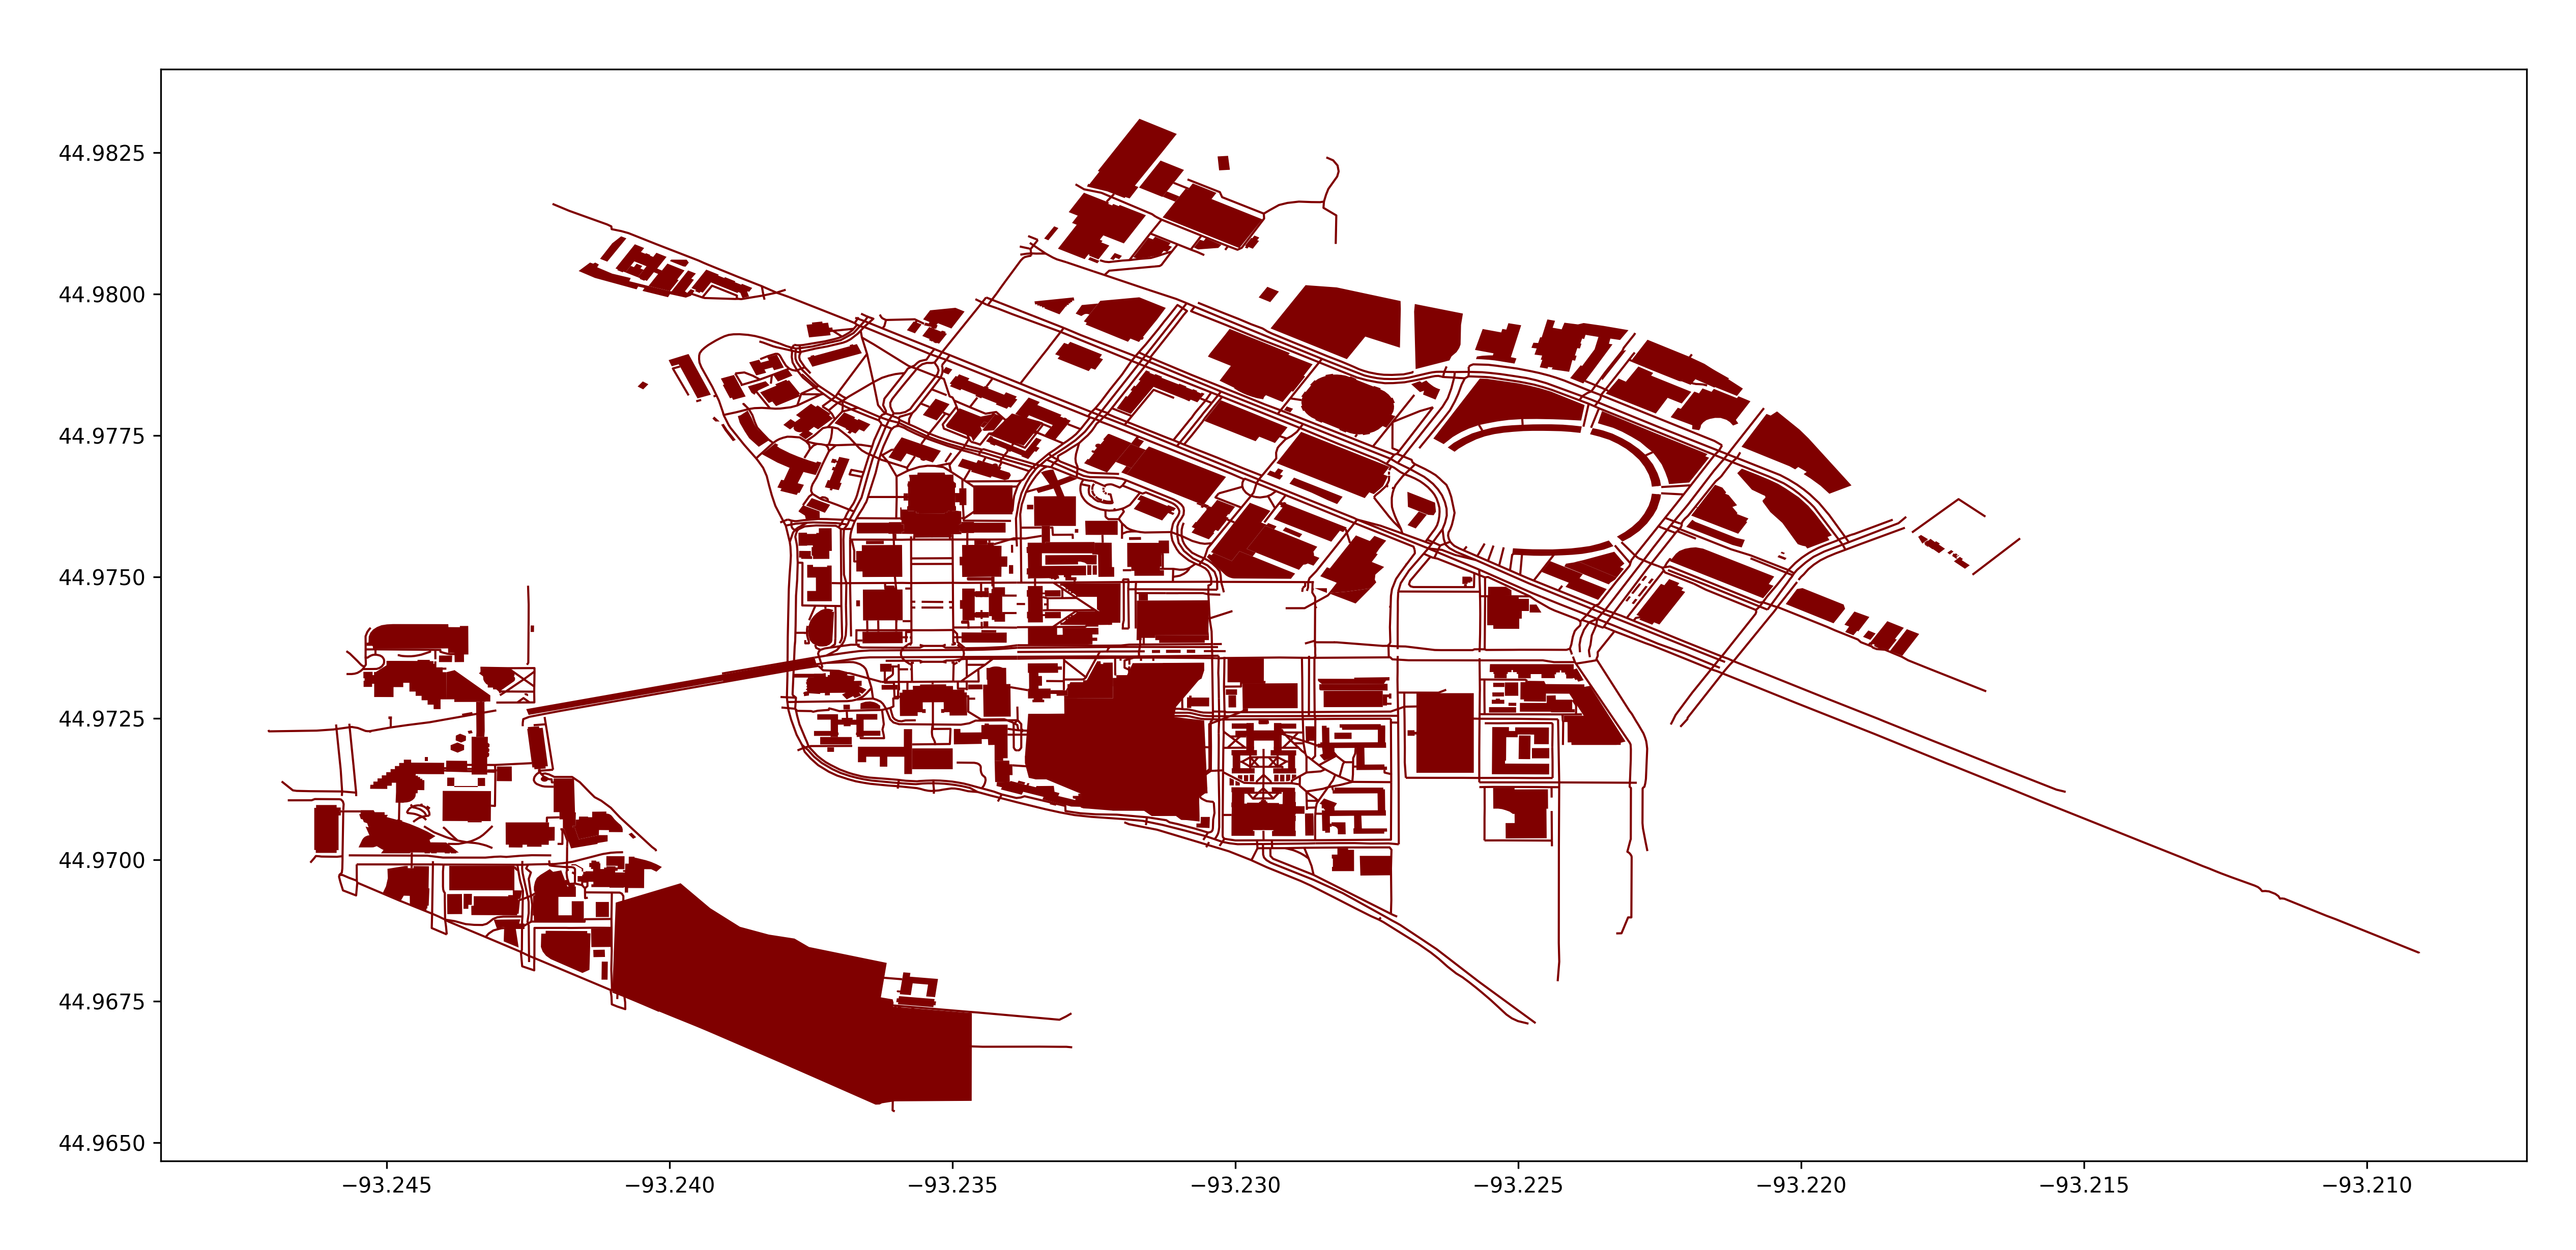
\includegraphics[scale=0.37]{images/complete_campus_map.png}
\caption{The Server's layer of the map.}
\label{fig: server's layer}
\end{figure}


Upon conducting a thorough literature review of the relevant algorithms, the decision was made to incorporate five algorithms, namely A* Algorithm, Breadth-First Search, Bidirectional Search, Dijkstra's Algorithm, and Bellman-Ford algorithm, into the program. Regarding A*, we will incorporate it with two heuristic functions, namely Manhattan distance and Haversine distance, to determine which one can more effectively enhance A*. It's worth noting that the weight on the graph is calculated by the Haversine distance for better accuracy of the distance on the map.

\begin{figure}[htbp]
\centering
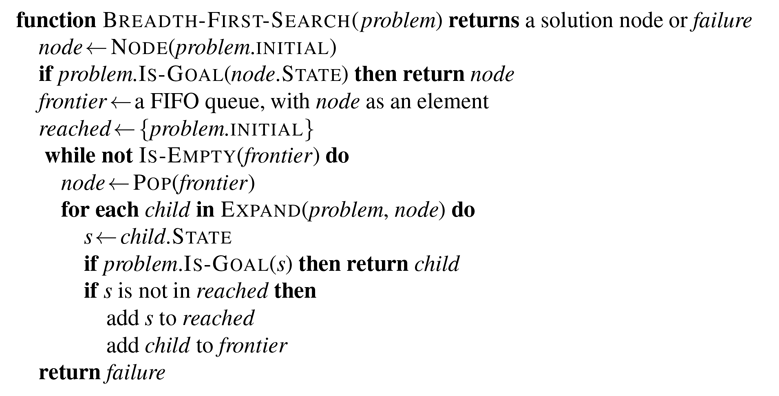
\includegraphics[scale=0.6]{images/BFS.png}
\caption{Breadth-First-Search algorithm pseudo-code in Artificial Intelligence 4th Edition\cite{Russell_Norvig_2021}}
\label{fig: bfs}
\end{figure}

\begin{figure}[htbp]
\centering
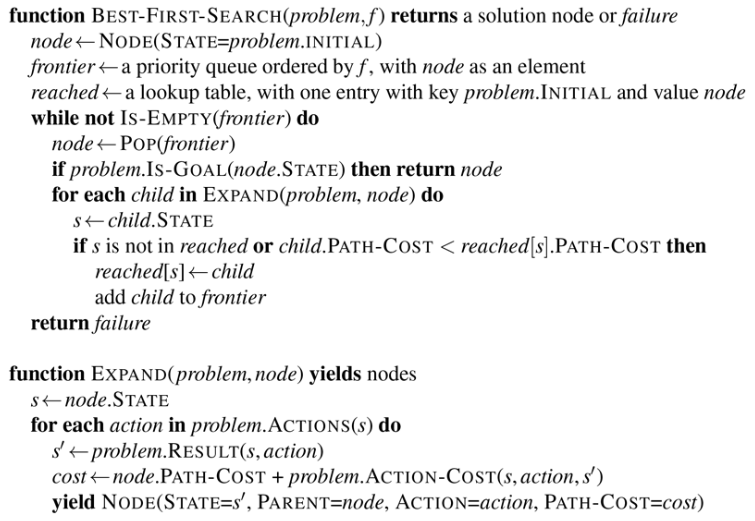
\includegraphics[scale=0.55]{images/Astar.png}
\caption{Best-First Search algorithm pseudo-code in Artificial Intelligence 4th Edition\cite{Russell_Norvig_2021}}
\label{fig: BF}
\end{figure}


The pseudo-codes outlined in the fourth edition of Artificial Intelligence were consulted (Figure \ref{fig: bfs} and \ref{fig: BF}), and based on these references, we implemented Breadth-First Search and A* Search both in Python and JavaScript. The A* Search is modified from the Best-First Search by using the evaluation function: \(f(n) = g(n) + h(n)\). Two heuristic functions, Manhattan Distance and Haversince Distance, are implemented for the A* algorithm. The Manhattan Distance is widely used in grid-based systems like Aziz's experiment \cite{Aziz_Anusha_Sheikh_2022}. It calculates the sum of the absolute differences between the horizontal and vertical coordinates. The Haversine function is typically used to find distances between two points on a sphere like the Earth, given their longitudes and latitudes. This makes it ideal for geographical applications, such as mapping and navigation systems. In our project, we plan to implement both of them to present a difference in efficiency in time and memory usage of the A* algorithm with two different heuristic functions. 

The experiment conducted by Fitro \cite{Fitro_2018} also employed the Dijkstra algorithm in the investigation of the shortest path problem between two points. In reference to the pseudo-code furnished by the study, we have implemented the Dijkstra algorithm in our program. For Bidirectional Search, we employed Breadth-First Search from two different starting points. Figure \ref{fig: bidirectional} presents the pseudo-code for the algorithm. In AbuSalim's comparative analysis\cite{AbuSalim_Ibrahim_Zainuri_Saringat_Jamel_Abdul_Wahab_2020}, the Bellman-Ford algorithm was utilized to address the Single-source shortest path problem. Following the provided code, we implemented the Bellman-Ford algorithm to find the shortest path between two points. The corresponding pseudo-code is presented in Figure \ref{fig: bellman-ford}.

Within the website's interface, a comprehensive menu comprising all the implemented algorithms is made available. This enables users to exercise their discretion in selecting the algorithm that best suits their preferences for route calculation.

We have devised three distinct methods for users to designate their origin and destination points. Specifically, users are afforded the option to either indicate a location by directly clicking on the map, inputting coordinates, or specifying building names. If a user identifies a point that does not lie on a roadway, the system will promptly compute and present the nearest roadway data point as a substitute for the user's initial selection.

The program can be operated in two distinct modes, namely Normal mode and Test mode. Upon selecting Normal mode, the program will employ the algorithm selected by the user to directly calculate the shortest path between the starting point and the ending point, subsequently displaying it on the map.

Alternatively, upon choosing Test mode, the program will execute the algorithm 100 times, recording the corresponding run time and memory usage of each instance. However, it has come to our attention that certain instances of memory usage can display negative values, attributed to underlying issues related to JavaScript and/or browser malfunctions. Such cases are appropriately labeled as "Invalid", and our function is designed to filter and disregard such invalid data points. In addition, the function presents the number of valid cases during each session, which is displayed on a pop-up window. Following the completion of the test, the program will display the shortest path length determined by the algorithm, the average run time, and the memory usage of the 100 trials.

\begin{figure}[H]
\centering
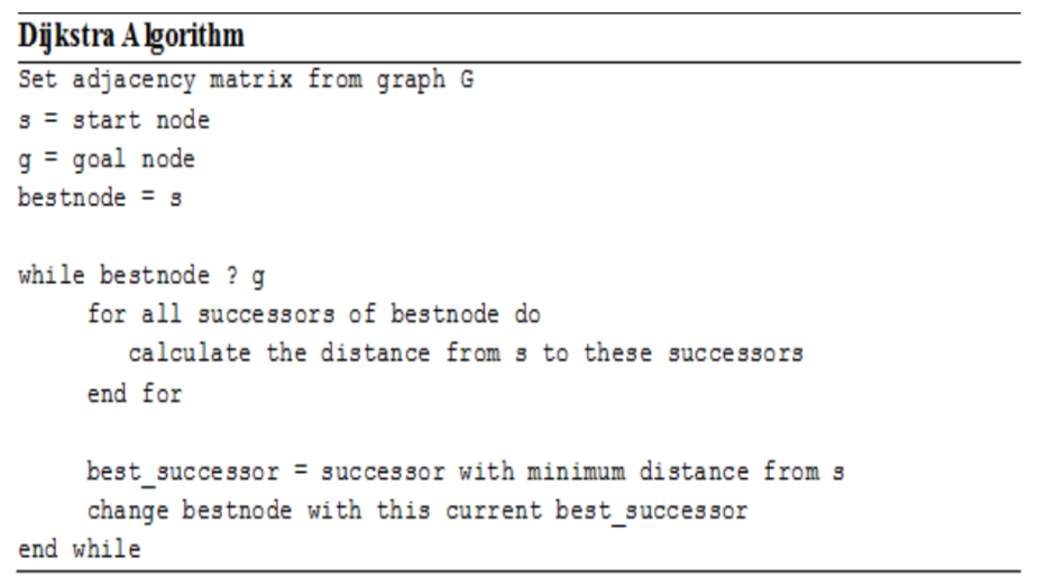
\includegraphics[scale=0.37]{images/Dijkstra(GIS).png}
\caption{Dijkstra Algorithm pseudo-code in Fitro’s experiment \cite{Fitro_2018}}
\label{fig: dijkstra}
\end{figure}

\begin{figure}[H]
\centering
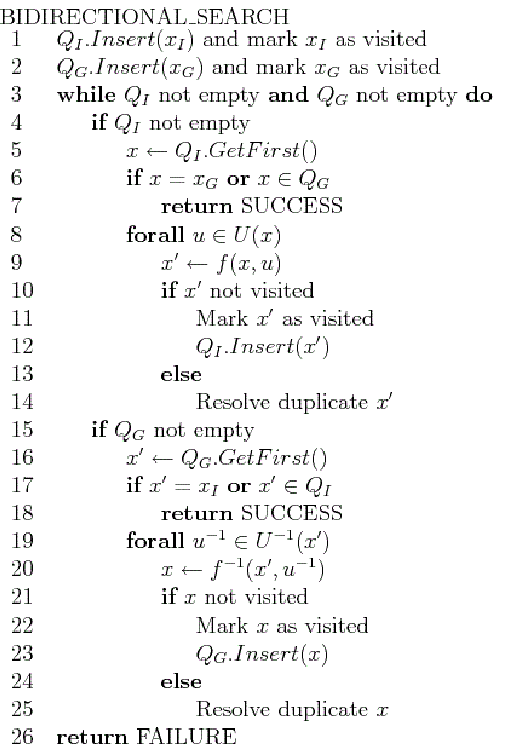
\includegraphics[scale=0.7]{images/BS.png}
\caption{pseudo-code for Bidirectional Search}
\label{fig: bidirectional}
\end{figure}

\begin{figure}[H]
\centering
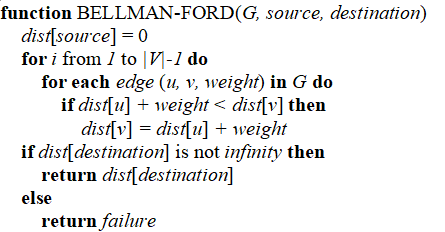
\includegraphics[scale=0.75]{images/BF.png}
\caption{pseudo-code for Bellman-Ford Search}
\label{fig: bellman-ford}
\end{figure}


\section{Experiment}

This section is organized into three distinct sections. The initial part details the experimental design, outlining the structure of the tests conducted, and elaborating on the methodologies employed for the collection and visualization of data. The second section presents the outcomes derived from the experimentation, coupled with comprehensive explanations for clarifying these findings. In the end, the last section provides an in-depth analysis of the aggregated results, a conclusive determination of the optimal choice among five algorithms, and a discussion of the limitations of the program and the experiment.

\subsection{Design}

Before the commencement of the experimental, we selected three distinct sets of origin and destination pairs. The first set encompassed departures from Anderson Hall (44.9723588, -93.2425962), with the destination being the University Recreation and Wellness Center (44.9751693, -93.2303338). The second group entailed departures from Eddy Hall (44.9777659, -93.2363017), with the destination being Frontier Hall (44.9712939, -93.2282896). Lastly, the third group involved departures from Walter Library (44.9752741, -93.2357297), with the destination being Boynton Health Service (44.9722088, -93.2340253).

In the experiment, we sequentially applied A* with Manhattan heuristic, A* with Haversine heuristic, Breadth-First search, Bidirectional Search, Dijkstra, and Bellman-Ford algorithm to calculate optimal paths between each set of origins and destinations. To mitigate potential errors, we activated the test mode of the program, wherein each algorithm undergoes 100 consecutive runs and returns averages of the results for enhanced accuracy and reliability. For each set of origins and destinations, we conducted 20 test runs for each algorithm and recorded the running time, memory usage, and route length in each run.

Subsequently, we analyzed the collected data and constructed histograms to represent the distribution of path lengths calculated by all algorithms for each group of locations. Additionally, we created line graphs to illustrate the running times and memory usage for each algorithm. This comprehensive visual representation allowed us to compare the performance of different algorithms more intuitively.

The outcomes for each table will be collected utilizing identical device, browser, and server settings. After the completion of data collection for a given table, the browser will undergo a refresh and be prepared for the subsequent table.

By adopting this rigorous approach, we aimed to provide a robust evaluation of the efficiency and effectiveness of the algorithms in our study. The utilization of multiple algorithms and repeated runs, along with the graphical representation of results, contributes to a deeper understanding of the comparative performance of these algorithms in the context of our study.


\subsection{Results}

This section discusses the results obtained from the aforementioned experiments. The aggregation of memory usage data stems from a non-standard feature named "enable-precise-memory-info" and is specific to the Chrome browser. It is worth noting that this approach may not be compatible with alternative web browsers.

During the experiment, our attention was initially directed toward the Bellman-Ford algorithm. While other algorithms typically complete calculations and yield results within 1-2 seconds, the Bellman-Ford algorithm required approximately thirty seconds to conclude a test run. As the disparity in the run-time and memory usage data between the Bellman-Ford algorithm and the other algorithms was significantly large, the former's data was excluded from the line chart to prevent it from adversely affecting the visual representation of the entire chart. Upon comparing the data of Bellman-Ford (Figure \ref{fig: bellman ford data}) with that of the other algorithms (Figure \ref{fig: avg time taken}, Figure \ref{fig: memory usage}), it was observed that the Bellman-Ford algorithm consumed almost a hundred times the resources used by the other algorithms. Consequently, it can be deduced that the Bellman-Ford algorithm necessitates a substantial amount of resources to function efficiently in this program. However, upon evaluating the paths computed by several algorithms (Figure \ref{fig: distance traveled}), it was found that Bellman-Ford produced the shortest path among all the algorithms employed in three experiments.

From a resource consumption standpoint, Bidirectional Search exhibits significantly lower data usage compared to other algorithms, positioning it as the fastest and most cost-effective option within the program. However, despite its expedient time and space performance, it yielded the worst path in all three experiments. This was particularly evident in the third experiment, where the generated path length was found to be twice that of other algorithms.

The Breadth-First Search algorithm also exhibits a notable degree of low resource occupancy rate, second only to the Bidirectional Search algorithm. However, in the first and third experiments, the path length as determined by Breadth-First Search is significantly lower than the path length computed by Bidirectional Search. Additionally, BFS consistently yields path lengths that are proximal to both the average and median values among all algorithms in all three experiments. It was a matter of surprise to us to observe that Breadth-First Search yielded comparable or superior results in comparison to the A* algorithm.

In each of the three experiments conducted, Dijkstra's algorithm computed routes that were highly comparable to those produced by the Bellman-Ford algorithm. While the route length of Dijkstra's algorithm was marginally greater than Breadth-First Search and A* in the third experiment, its routes in the first and second experiments were significantly more optimal than those generated by the former two algorithms. In terms of resource occupancy, Dijkstra's algorithm ranks second to Bellman-Ford. However, the time and space performance of Dijkstra's algorithm is only marginally inferior to that of other algorithms and is not characterized by a significant gap in performance, as is the case with Bellman-Ford.

The empirical analysis shows that A* algorithm's run-time and memory usage are comparable to the mean performance. Specifically, the overall resource consumption of A* algorithm with Haversine heuristic is marginally higher than that of A* algorithm with Manhattan heuristic. Nevertheless, the discrepancy is insignificant. Furthermore, the computational time of both A* algorithms is marginally higher than Breadth-First Search algorithm. The memory utilization of A* algorithms is twice that of Breadth-First Search. Both heuristic functions in A* algorithm yield the same optimal path. In the first experiment, the route computed by Breadth-First Search outperformed the one computed by A*. In the other two experiments, BFS and A* returned the same results.

\begin{figure}[H]
\centering
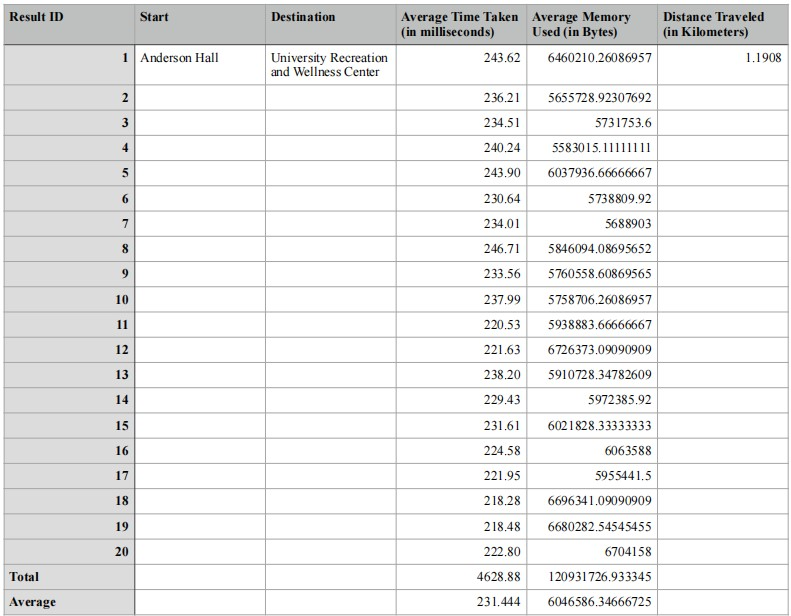
\includegraphics[scale=0.6]{images/bf test1.jpg}
\caption{The results of the Bellman-Ford algorithm on Test 1}
\label{fig: bellman ford data}
\end{figure}

\begin{figure}[H]
\centering
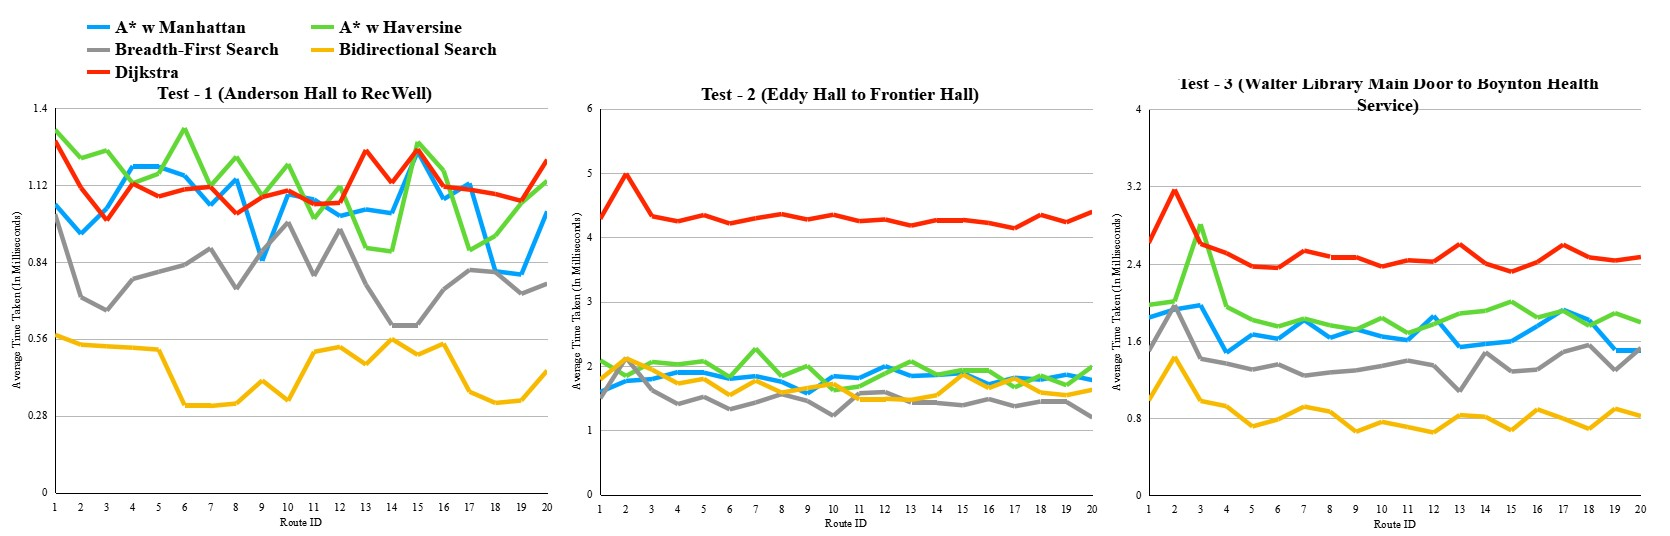
\includegraphics[scale=0.37]{images/time taken data.jpg}
\caption{The average running time of five algorithms in three tests. The x-axis is the id of the 20 trials. The y-axis is the average time taken (in Milliseconds)}
\label{fig: avg time taken}
\end{figure}

\begin{figure}[H]
\centering
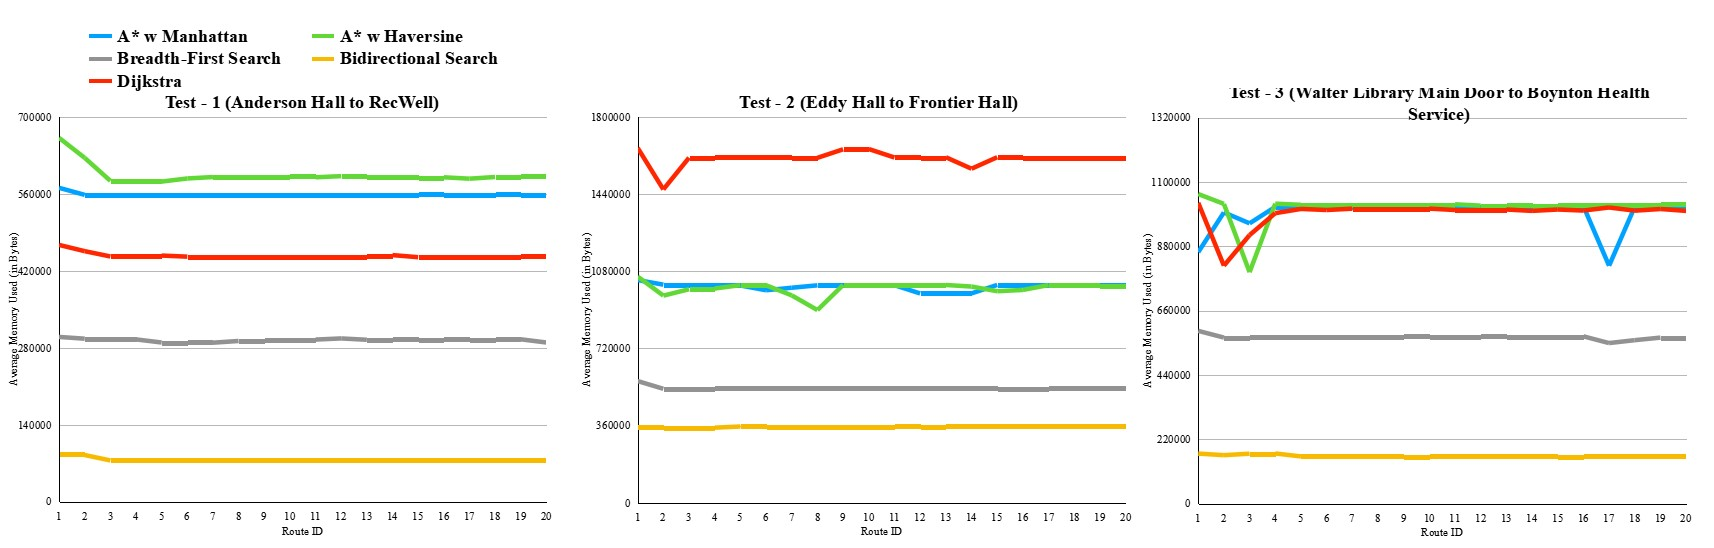
\includegraphics[scale=0.36]{images/memory usage data.jpg}
\caption{The average memory used of five algorithms in three tests. The x-axis is the id of the 20 trials. The y-axis is the average memory used (in Bytes)}
\label{fig: memory usage}
\end{figure}

\begin{figure}[H]
\centering
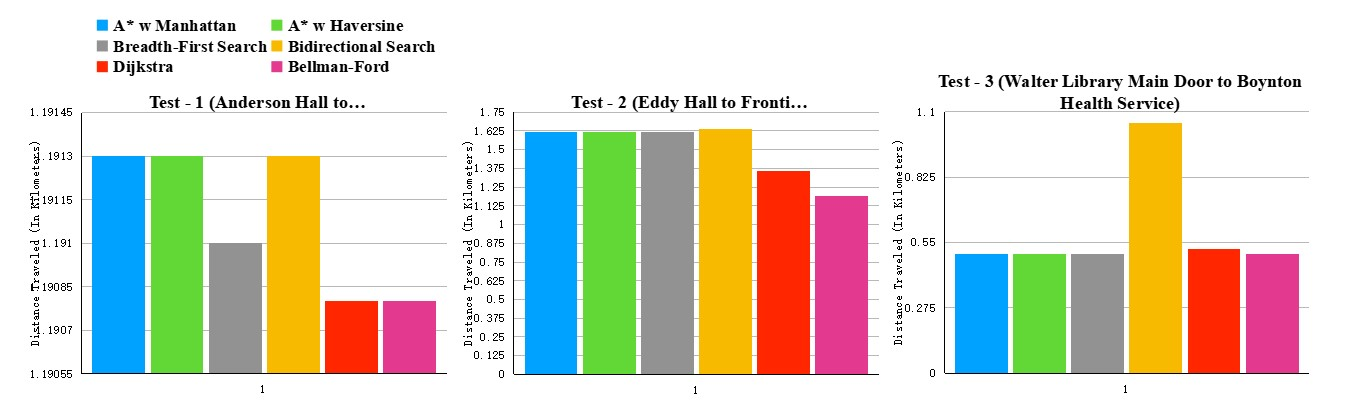
\includegraphics[scale=0.45]{images/distance data.jpg}
\caption{The distance of the shortest path found by algorithms in three tests. The x-axis is the id of the 20 trials. The y-axis is the distance of the shortest path obtained (in Kilometers)}
\label{fig: distance traveled}
\end{figure}


\subsection{Analysis}

\subsubsection{Optimal Path}

Based on the experimental results, the Bellman-Ford algorithm appears to be the optimal choice for finding the optimal path in this program. Although its CPU running time is considerably longer than other algorithms during the test, in the Normal mode, which is provided to users and does not require as many runs as the Test mode, the time gap in planning the route can be overlooked. The inferior time and space performance of Bellman-Ford can be attributed to the immense size of the graph of the UMN map. In AbuSalim's comparative analysis \cite{AbuSalim_Ibrahim_Zainuri_Saringat_Jamel_Abdul_Wahab_2020}, there were also cases where the Bellman-Ford running time increased disproportionately as the number of nodes increased exponentially. This can be attributed to its time complexity of \(O(|V|*|E|)\). As noted in our literature review, Bellman-Ford yields better results on smaller graphs.

As anticipated, the Dijkstra algorithm can also be one of the most recommended methods in this program. As elucidated by Fitro\cite{Fitro_2018} and Wayahdi\cite{Wayahdi_2021_GreedyAA}, it should be noted that the Dijkstra algorithm may necessitate additional time and memory resources for finding the optimal solution, relative to other algorithms. Nevertheless, when compared to the computational resources required by the Bellman-Ford algorithm, the resource consumption of Dijkstra is relatively inconsequential. Despite this, the Dijkstra algorithm remains capable of producing results that are highly comparable to those obtained by the Bellman-Ford algorithm.

The performance of the A* algorithm in this experiment was unexpected. The findings of both Aziz\cite{Aziz_Anusha_Sheikh_2022} and Zeng\cite{Zeng_Church_2009} suggest that A* outperforms Dijkstra's algorithm. However, it did not achieve the anticipated level of performance. As observed in Wayahdi's experimental findings\cite{Wayahdi_2021_GreedyAA}, in most scenarios, Dijkstra yielded a more optimal path than A*. We attribute this observation to the unsuitability of the A* algorithm for the map pattern of UMN, as the heuristic calculated based on this map does not effectively contribute to the algorithm's computations, thereby resulting in sub-optimal outcomes.

The disparity among Breadth-First Search, Bidirectional Search, and other algorithms is relatively narrower than anticipated. Nevertheless, these algorithms are not well-suited as the recommendation algorithm of this program. Excluding A* due to its inability to function normally, one can observe that paths returned by Breadth-First Search and Bidirectional Search are noticeably sub-optimal compared to Bellman-Ford and Dijkstra. Although their short run-time and minimal memory usage are advantageous, they compromised the optimality of the outcomes as a trade-off.


\subsubsection{Limitation}

As Figure \ref{fig: server's layer} depicts, the actual size of the map for algorithms is limited, i.e., there could be more paths that can be walked in the real world. The elevation of some paths in the West Bank of the campus also becomes an obstacle for the program to find the shortest path there and decreases the probability of finding the shortest path successfully, since the map is two-dimensional.

Despite our efforts to maintain accuracy and consistency in the results by excluding invalid cases and averaging our data, the performance measurement of the algorithms still presents certain limitations. These are primarily associated with JavaScript and its garbage collection system, especially when monitoring memory usage. These issues could potentially skew the results of the experiment, thus representing the biggest limitation of our project.


\section{Conclusion}

To assist students at the University of Minnesota (UMN) in navigating around campus, we designed a program that offers more detailed navigation than traditional methods. The program permits users to choose their starting point and destination on the UMN map and offers various algorithms to calculate routes. Specifically, this program incorporates six algorithms, namely A* with Manhattan, A* with Haversine, Breadth-First Search, Bidirectional Search, Dijkstra Algorithm, and Bellman-Ford Algorithm.

Following the completion of the program's development, a thorough testing and evaluation of the six algorithms was conducted on the UMN campus map. The results indicate that Bellman-Ford and Dijkstra are the most appropriate algorithms for application on this map. Of the two, the Bellman-Ford algorithm provides an optimal path, while the Dijkstra algorithm can calculate paths of comparable length using fewer resources than Bellman-Ford. Breadth-First Search and Bidirectional Search are less resource-intensive but produce sub-optimal paths. The results deemed A* unsuitable for use with this map, as its results were inferior to those obtained with Dijkstra and Breadth-First Search.

If this project will undergo further development in the future, we will give due consideration to augmenting it with additional architectural features such as doorways, internal structures, stairs, and underground passages to optimize route efficiency. It is noteworthy that several of the academic buildings at UMN are interlinked through subterranean pathways, and we anticipate that the inclusion of underpasses in our project will pave the way for new and more optimal routes. In addition, we aim to enhance the overall user experience by providing a 3D view of the routes, thereby augmenting their visual clarity and intuitiveness.


\section{Contribution}

Our source code \footnote{\url{https://github.umn.edu/WANG9747/umn-csci4511w-final-project}} is available via GitHub Enterprise. 
Here is how we separate all the work:
\begin{table}[hbt!]
\centering
\begin{tabular}{|p{6cm}|p{3cm}|p{3cm}|} \hline
\multicolumn{3}{|c|}{\textbf{Project}} \\ \hline
\textbf{Tasks} & \textbf{People} & \textbf{Reviewed By} \\ \hline
Literature review                                       & Yicheng Zhai & Junyuan Wang \\ \hline
OSM data collection, cleaning, and processing           & Junyuan Wang & Yicheng Zhai \\ \hline
Graph Creation                                          & Junyuan Wang & Yicheng Zhai \\ \hline
Algorithms Implementation                               & Yicheng Zhai & Junyuan Wang \\ \hline
App setup                                               & Junyuan Wang & Yicheng Zhai \\ \hline
Performance measurement                                 & Junyuan Wang & Yicheng Zhai \\ \hline
Result visualization                                    & Yicheng Zhai & Junyuan Wang \\ \hline
Final Report                                            & Yicheng Zhai & Junyuan Wang \\ \hline
\end{tabular}
\end{table}

\newpage
\printbibliography

\end{document}
